%----------------------------------------------------------------------
\begin{frame}[c]{Where are we? The big picture}

\begin{itemize}
\item Algorithm Selection
  \begin{itemize}
    \item Portfolios
    \item Algorithm selection (for runtime)
  \end{itemize}
  \item Design decisions:\\ Local Search + Evo. Algorithms + Machine Learning 
  \item Empirical evaluation
  \item AAD for ML
  \begin{itemize}
    \item Hyperparameter optimization and Bayesian optimization 
    \item Neural architecture search (lecture given by Prof. Hutter)
  \end{itemize}
  \item Algorithm configuration 
  \begin{itemize}
    \item Basics 
    \item State of the art 
    \item Best practices 
  \end{itemize}
  \item Combinations of algorithm selection and configurations
  \item Algorithm control and learning to learn
  \item[$\to$] Algorithm analysis 
  \item Project announcement and questions for exam 
\end{itemize}

\end{frame}
%----------------------------------------------------------------------
%----------------------------------------------------------------------
\begin{frame}[c]{Learning Goals}

After this lecture, you will be able to \ldots

\begin{itemize}
  \item use data gathered for algorithm configuration to gain more insights about the algorithm and instances
  \item distinguish between global and local parameter importance
  \item explain parameter importance for the following approaches:
  \begin{itemize}
    \item fANOVA
    \item Ablation studies
    \item Forward selection
    \item Local parameter importance (LPI)
  \end{itemize}
  \item understand and use performance analysis approaches\\ (incl. algorithm footprints)
  \item understand and use configurator analysis\\ (e.g., performance over time and algorithm configurator footprints)
\end{itemize}

\end{frame}
%----------------------------------------------------------------------
%----------------------------------------------------------------------
\begin{frame}[c]{Main Reference}

Main reference for today: \\
\href{https://ml.informatik.uni-freiburg.de/papers/18-LION12-CAVE.pdf}{\textit{CAVE: Configuration Assessment, Visualization and Evaluation}}
\\by Biedenkapp, Lindauer and Hutter (LION'18)

\bigskip
Our reference implementation
\url{https://github.com/automl/CAVE}

\bigskip

Goal for today:\\
Understand how CAVE works and how to use it!


\end{frame}
%----------------------------------------------------------------------
\begin{frame}[c]{Empirical Algorithm Analysis}

\begin{block}{Idea}
\begin{itemize}
  \item We collect a lot of performance data for all our approaches
  \begin{itemize}
    \item algorithm selection, hyperparameter optimization, algorithm configuration, algorithm control
  \end{itemize}
  \pause
  \item so far we asked only: how to improve the performance of algorithms
  \pause
  \item but can we do more with all the data?
  \pause
  \item[$\leadsto$] use performance data to analyze algorithms (and instances)
\end{itemize}

\end{block}

\end{frame}
%----------------------------------------------------------------------
%----------------------------------------------------------------------
\begin{frame}[c]{Algorithm Analysis Workflow}

\scalebox{0.75}{
\tikzset{reset preactions/.code={\def\tikz@preactions{}}}
\makeatother
\tikzstyle{activity}=[rectangle, draw=black, rounded corners, text centered, text width=6em, fill=white, drop shadow]
\tikzstyle{data}=[rectangle, draw=black, text centered, fill=black!10, text width=8em, drop shadow]
\tikzstyle{myarrow}=[->, thick]
\begin{tikzpicture}[node distance=8em]
	
	
	\node (TA) [data, text width=10em] {Algorithm $\algo$ with Config. Space $\pcs$};
	\node (Insts) [data, text width=10em, below of=TA, node distance=4em] {Instance set $\insts$\\ (with Features $\feat(\inst)$)};
	\node (P) [data, text width=10em, below of=Insts, node distance=4em] {Cost metric\\ $c: \pcs \times \insts \to \perf$};
	
	\node (AC3) [activity, text width=6em, right of=Insts, node distance=10em, yshift=0.6em, xshift=0.6em, reset preactions] {Configuration\\ (e.g., SMAC)};
	\node (AC2) [activity, text width=6em, right of=Insts, node distance=10em, yshift=0.3em, xshift=0.3em, reset preactions] {Configuration\\ (e.g., SMAC)};
	\node (AC) [activity, text width=6em, right of=Insts, node distance=10em, yshift=0em, reset preactions] {Configuration\\ (e.g., SMAC)};
	
	\node (Traj) [data, text width=7.6em, right of=AC, node distance=10em, yshift=4em] {Trajectories\\ $\langle \hat{\conf}_i, t_i\rangle_i$};
	\node (Runhistory) [data, text width=7.6em, right of=AC, node distance=10em] {Runhistories\\ $\{ \conf_j, \inst_j, c(\conf_j, \inst_j)\}_j^N$};
	\node (EPM) [data, text width=7.6em, right of=AC, node distance=10em, yshift=-4em] {EPM\\$\surro: \pcs \times \insts \to \perf$};
	
	\node (Perf) [activity, text width=7em, right of=Traj, node distance=10.5em] {Performance Analysis};
	\node (Feature) [activity, text width=7em, right of=Runhistory, node distance=10.5em] {Feature Analysis};
	\node (PIMP) [activity, text width=7em, right of=EPM, node distance=10.5em] {Parameter Importance};
	\node (Beh) [activity, text width=7em, right of=EPM, node distance=10.5em, yshift=-4em] {Configurator Behavior};
	
	
	\draw[myarrow] ($(AC.west)+(-0.3,0)$) -- (AC);
	
	\draw[myarrow] ($(AC.east)+(0.2,0)$) -- ($(Runhistory.west)+(-0.33,0)$);
	\draw[myarrow, dashed] (Runhistory) -- (EPM) node [right, yshift=1.85em] {Train};
	
	\draw[myarrow] ($(Runhistory.east)+(0.35,0)$) -- ($(Feature.west)+(-0.11,0)$);
	
%	\draw[myarrow] (Inst3) -- (Conf3);
%	\draw[myarrow] ($(Conf2)+(0,-0.8)$) -- (Conf3) node[right, yshift=3.7em] {$\hist^1 \cup \hist^2$};
	
	
	\begin{pgfonlayer}{background}

    	\path (TA -| TA.west)+(-0.1,0.8) node (resUL) {};
    	\path (P.east |- P.south)+(0.1,-0.5) node(resBR) {};
    	\path [rounded corners, dashed, draw=black!50] (resUL) rectangle (resBR);
		\path (P.east |- P.south)+(-1.6,-0.35) node [text=black!80] {Configurator's Input};

		\path (Perf -| Perf.west)+(-0.1,0.8) node (resUL2) {};
    	\path (Beh.east |- Beh.south)+(0.1,-0.5) node(resBR2) {};
    	\path [rounded corners, dashed, draw=black!50] (resUL2) rectangle (resBR2);
		\path (Beh.east |- Beh.south)+(-0.425,-0.35) node [text=black!80] {CAVE};

		\path (Traj -| Traj.west)+(-0.33,0.8) node (resUL3) {};
    	\path (EPM.east |- EPM.south)+(0.33,-1.0) node(resBR3) {};
    	\path [rounded corners, dashed, draw=black!50] (resUL3) rectangle (resBR3);
		\path (EPM.east |- EPM.south)+(-1.5,-0.45) node [text=black!80] {Configurator's Output };
		\path (EPM.east |- EPM.south)+(-.85,-0.85) node [text=black!80] {CAVE's Input};
		

    \end{pgfonlayer}
	
\end{tikzpicture}

}

\end{frame}
%----------------------------------------------------------------------
%----------------------------------------------------------------------
\begin{frame}[c]{Reminder: Performance Analysis}

\begin{columns}
\column{0.33\textwidth}
\includegraphics[width=1\textwidth]{images/crafted_CSSC-Queens-300s-2day_clasp-3_0_4-p8}
\centering
Scatter Plot
\column{0.33\textwidth}
\includegraphics[width=1\textwidth]{scripts/runtime_plots/cdf_test_clasp_queens.png}
\centering
CDF Plot
\column{0.33\textwidth}
\includegraphics[width=1\textwidth]{images/footprint_spear_swv}
\centering
Algorithm Footprints
\end{columns}

\pause
\bigskip

\begin{itemize}
  \item \alert{Insight:} Optimized configuration has a better performance\\ on nearly all instances
\end{itemize}

\end{frame}
%----------------------------------------------------------------------
%----------------------------------------------------------------------
\begin{frame}[c]{Feature Analysis: Feature Correlation}

\begin{itemize}
  \item Correlated features can hurt some ML approaches
  \item Wasted time to compute correlated features
\end{itemize}

\centering
\includegraphics[width=0.6\textwidth]{images/feature_correlation}

\pause
\smallskip

\begin{itemize}
  \item \alert{Insight:} Many features are highly correlated
\end{itemize}

\end{frame}
%----------------------------------------------------------------------
%----------------------------------------------------------------------
\begin{frame}[c]{Feature Analysis: Violin and Box Plots}

\begin{itemize}
  \item Study instance features can help to understand instance distribution
  \begin{itemize}
    \item Are all distributions unimodal? $\to$ higher chance of homogeinity 
    \item Are some distributions multimodal? $\to$ higher chance of heterogeneity 
  \end{itemize}
\end{itemize}

\centering
\includegraphics[width=0.9\textwidth]{images/violin_box_nvarsOrig_plot}

\#number of variables in SAT problem

\end{frame}
%----------------------------------------------------------------------
%----------------------------------------------------------------------
\begin{frame}[c]{Feature Analysis: Clustering}

\begin{itemize}
  \item Cluster instances to study the joint instance feature distribution
  \item Could also provide evidence for heterogeneity
\end{itemize}

\centering
\includegraphics[width=0.68\textwidth]{images/instance_clustering}
%spear_swv

\pause
\smallskip

\begin{itemize}
  \item \alert{Insight:} Most instances belong to one cluster
\end{itemize}

\end{frame}
%----------------------------------------------------------------------
%----------------------------------------------------------------------
\begin{frame}[c]{Algorithm Parameter Importance}

\begin{block}{Observation}
\begin{itemize}
  \item We recommend to configure all parameters that could influence performance
  \pause
  \item However, often only a few parameter matter
  \pause 
  \item Dependent on the instance set, different parameters matter \lit{Biedenkapp et al. 2018}
  \pause
  \item[$\leadsto$] \alert{How to determine the algorithm parameter importance}?
\end{itemize}
\end{block}

\medskip
\pause

\begin{block}{Example}
\begin{itemize}
  \item the SAT solver \lingeling{} has more than $300$ parameters
  \item Often, less than $10$ are important to optimize performance
\end{itemize}
\end{block}


\end{frame}
%----------------------------------------------------------------------
%----------------------------------------------------------------------
\begin{frame}[c]{Ablation~\litw{C. Fawcett et al. 2013}}

\small
\begin{block}{Idea}
\begin{itemize}
  \item Starting from the default configuration, we change the value of the parameters
  \item Which of these changes were important?
  \item[$\to$] Ablation compares parameter flips between default and incumbent configuration  
\end{itemize}
\end{block}

\pause

\begin{block}{Basic Approach}
\begin{itemize}
  \item Iterate over all non-flipped parameters
  \item Flip the parameter with the largest influence on the performance in each iteration
\end{itemize}
\end{block}
 
\end{frame}
%----------------------------------------------------------------------
%----------------------------------------------------------------------
\begin{frame}[c,fragile]{Ablation Pseudo Code}

\LinesNotNumbered
\begin{algorithm}[H]
\Input{%
instance set $\insts$,
Algorithm $\algo$ with configuration space $\confs$,
start configuration $\conf_0$,
target configuration $\conf_t$, metric $c$,
}
\BlankLine
$\conf \leftarrow  \conf_0$; \\
$C \leftarrow [] $ ;\\ 
\ForEach{$i \in \{1 \ldots |\pcs|\}$}{
	\ForEach{$\delta \in \Delta(\conf, \conf_t)$}{
		$\conf'$ $\leftarrow$ apply $\delta$ to $\conf$;\\
		evaluate $c(\delta) = \sum_{\inst \in \insts} c(\conf',\inst)$;
	}
	Determine most important change $\delta^* \in \argmin_{\delta \in \Delta(\conf, \conf_t)} c(\delta)$;\\
	$\conf$ $\leftarrow$ apply $\delta^*$ to $\conf$;\\
	C.append($\delta^*);\\
}
\pause
\Return{$C$}
\caption{Ablation}
\end{algorithm}

\end{frame}
%----------------------------------------------------------------------
%----------------------------------------------------------------------
\begin{frame}[c,fragile]{Toy example: Ablation}

\centering
\small
\begin{tabular}{l ccc c}
\toprule
 		& $\conf_1$ & $\conf_2$ & $\conf_3$ & $m$\\
\midrule
Default & 1 & 1 & 1 & $100$\\
Conf & 2 & 2 & 2 & $10$\\
\hline
\pause
\textbf{1st Iteration}\\
		& 2 & 1 & 1 & $90$ \\
		& 1 & 2 & 1 & $30$ \\
		& 1 & 1 & 2 & $100$ \\
$\leadsto$ Flip $\conf_2$\\
\hline
\pause
\textbf{2nd Iteration}\\
		& 2 & 2 & 1 & $10$ \\
		& 1 & 2 & 2 & $30$ \\
$\leadsto$ Flip $\conf_1$\\
\hline
\pause
\textbf{3rd Iteration}\\
		& 2 & 2 & 2 & $10$ \\
$\leadsto$ Flip $\conf_3$\\
\bottomrule
\end{tabular}

\end{frame}
%----------------------------------------------------------------------
%----------------------------------------------------------------------
\begin{frame}[c]{Ablation Example: \textit{Spear} on SWV}

\centering
\includegraphics[width=.8\textwidth]{images/ablation_spear_swv}

\small
\centering
Source: \lit{C. Fawcett et al. 2013}
\end{frame}
%----------------------------------------------------------------------
%----------------------------------------------------------------------
\begin{frame}[c]{Ablation: Improvements}

\begin{block}{Improvement Ablation with Racing}
\begin{itemize}
  \item To determine the best flip in each iteration,
  		use \alert{racing} with a statistical test to speed up the decision
  \item[$\to$] do not assess the performance on all instances
\end{itemize}
\end{block}

\pause

\begin{block}{Ablation with Performance predictions}
\begin{itemize}
  \item Use gathered performance data from algorithm control
  \item Train empirical performance model (EPM) on this data
  \item Use EPM instead of new, expensive algorithm runs
\end{itemize}
\end{block}

\end{frame}

%----------------------------------------------------------------------
%----------------------------------------------------------------------
\begin{frame}[c]{Ablation: Summary}

\begin{itemize}
  \item Local parameter importance analysis: Comparing two configurations
  \pause
  \medskip
  \item Helps to explain why a configurator made some changes
  \pause
  \medskip
  \item Disadvantages:
  \begin{itemize}
    \item Interactions between parameters are ignored
    \item Expensive to run because many new algorithm runs are required
  \end{itemize}
\end{itemize}

\end{frame}
%----------------------------------------------------------------------
%----------------------------------------------------------------------
\begin{frame}[c]{Local Paramter Importance (LPI)~\litw{Biedenkapp et al. 2018}}

\begin{block}{LPI}
\begin{itemize}
  \item Human strategy: Study final incumbent $\hat{\conf}$ by changing each parameter seperately
  \smallskip
  \pause
  \item LPI does the same but based on EPMs 
\end{itemize}

\centering
\includegraphics[width=0.55\textwidth]{images/lpi-sp-clause-decay_log}
\end{block}

\end{frame}
%----------------------------------------------------------------------
%----------------------------------------------------------------------
\begin{frame}[c]{Local Paramter Importance (LPI)~\litw{Biedenkapp et al. 2018}}

\begin{block}{LPI: Importance of each Parameter}
\begin{itemize}
  \item Quantify importance by impact of changing parameter value on performance
  \item Given: parameter $p \in P$, parameter domain $\pcs_p$,\\ configuration $\conf$, marginalized EPM $\surro: \pcs \to \perf $ 
\end{itemize}
\[LPI(p \mid \theta) = \frac{\mathrm{Var}_{v\in\pcs_p}\surro(\conf\left[\conf_p=v\right])}{\sum_{p'\in P}\mathrm{Var}_{w\in\pcs_{p'}}\surro(\conf\left[\conf_{p'}=w\right])}\]
\end{block}

\pause

\begin{block}{Summary}
\begin{itemize}
  \item Even more local than Ablation
  \item Accuracy depends on EPM
  \item Disadvantage: Ignores interactions between parameters 
\end{itemize}
\end{block}

\end{frame}
%----------------------------------------------------------------------
%----------------------------------------------------------------------
\begin{frame}[c]{Forward Selection~\litw{F. Hutter et al. 2013}}

\begin{block}{Idea}
\begin{itemize}
  \item Which parameters (or instance features) do we need \\to train a good EPM ($\hat{m}: \pcs \times \insts \to \perf$)?
  \item Use \alert{forward selection} to identify important parameters (/instances)
  \item (Also ignores interaction effects) 
\end{itemize} 
\end{block}

\pause
\medskip

\begin{block}{Details}
\begin{itemize}
  \item Minimize RMSE (root mean squared error) on a validation set
  \item Limit the maximal number of selected parameters (/features) 
\end{itemize} 
\end{block}

\end{frame}
%----------------------------------------------------------------------
%----------------------------------------------------------------------
\begin{frame}[c]{Forward Selection}

\LinesNotNumbered
\begin{algorithm}[H]
\Input{%
instance set $\insts$,
Algorithm $\algo$ with configuration space $\confs$,\\
set of parameters $P$, metric $c$,\\
trainig data set $\mathcal{D}_{\text{train}} = \langle (\conf_i, \inst_i), c(\conf_i,\inst_i) \rangle^N$,\\
validation data set $\mathcal{D}_{\text{val}} = \langle (\conf_i, \inst_i), c(\conf_i,\inst_i) \rangle^K$,
}
\BlankLine
$P' \leftarrow [] $ ;\\ 
\ForEach{$i \in \{1 \ldots |P|\}$}{
	\pause
	\ForEach{$p \in P - P'$}{
		train EPM on $\mathcal{D}_{\text{train}}$ limited to $P' \cup \{p\} \times \insts$;\\
		evaluate EPM on $\mathcal{D}_{\text{val}}$;
	}
	\pause
	Determine most important change $p$ according to validation RMSE;\\
	$P'$.append($p$);\\
}
\pause
\Return{$P'$}
\caption{Forward Selection}
\end{algorithm}

\end{frame}
%----------------------------------------------------------------------
%----------------------------------------------------------------------
\begin{frame}[c]{Forward Selection~\litw{F. Hutter et al. 2013}}

\centering
Spear on SWV\\
\includegraphics[width=0.6\textwidth]{images/forward_sel_spear_swv.png}

\end{frame}
%----------------------------------------------------------------------
%----------------------------------------------------------------------
\begin{frame}[c]{\fanova{}~\litw{F. Hutter et al. 2014}}

\begin{block}{\fanova{}~\litw{Sobobl 1993}}
Write performance predictions as a sum of components:
\begin{eqnarray}
 \hat{y}(\conf_1,\ldots,\conf_n) =& \hat{f}_0 + \sum_{i=1}^{n} \hat{f}_i(\conf_i) + \sum_{i \neq j} \hat{f}_{ij}(\conf_i,\conf_j) + \ldots \nonumber \\
 \hat{y}(\conf_1,\ldots,\conf_n) =& \text{average response} + \text{main effects} +\nonumber\\ &\text{2-D interaction effects} + \text{higher order effects} \nonumber
\end{eqnarray}
\end{block}

\pause

\begin{block}{Variance Decomposition}
\begin{equation}
\mathrm{V} = \frac{1}{||\confs||} \int_{\conf_1} \ldots \int_{\conf_n} [(\hat{y}(\conf)- \hat{f}_0)^2] d\conf_1 \ldots d\conf_n\nonumber
\end{equation}
\end{block}

\pause

\begin{block}{Application to Parameter Importance}
How much of the variance can be explained by a parameter (or combinations of paramaters) marginalized over all other parameters?
\end{block}

\end{frame}
%----------------------------------------------------------------------
%----------------------------------------------------------------------
\begin{frame}[c]{\fanova{} Example}

\centering
\lingeling{} on circuit fuzz

\includegraphics[scale=0.4]{images/fanova-lingeling-circut_fuzz_cssc14.png}

\end{frame}
%----------------------------------------------------------------------
%----------------------------------------------------------------------
\begin{frame}[c]{\fanova{} Example}

\centering
\lingeling{} on circuit fuzz

\includegraphics[scale=0.3]{images/fanova_lingeling_score_cf}

$0$ seems to be a worse value for \texttt{score}

\end{frame}
%----------------------------------------------------------------------
%----------------------------------------------------------------------
\begin{frame}[c]{\fanova{} Example}

\begin{block}{Interesting part of the configuration space}
Consider only performance values better than the default ($c(\conf) \leq c(\conf_0)$)
\end{block}

\centering
\lingeling{} on circuit fuzz

\includegraphics[scale=0.25]{images/fanova-lingeling-circut_fuzz_cssc14_defcut}

\end{frame}
%----------------------------------------------------------------------
% %----------------------------------------------------------------------
% \begin{frame}[c]{\fanova{} Example}
% 
% \centering
% \lingeling{} on circuit fuzz
% 
% \includegraphics[scale=0.3]{images/fanova-lingeling-circut_fuzz_cssc14_defcut_decolim}
% 
% \end{frame}
% %----------------------------------------------------------------------
%----------------------------------------------------------------------
\begin{frame}[c]{\fanova{} Example}

\centering
\textit{probSAT} on 3-SAT instances

\includegraphics[scale=0.22]{images/fanova_probsat_3sat_cssc14_cb1}

\bigskip
The red-shaded area indicates the uncertainty of the model.

\end{frame}
%----------------------------------------------------------------------
%----------------------------------------------------------------------
\begin{frame}[c]{Comparison Ablation, Forward Selection \& \fanova{}}

\small
\begin{block}{Ablation + LPI}
\begin{itemize}
  \item[+] Local analysis -- easy to interpret
  \item[-] No interaction effects  
\end{itemize}
\end{block}

\vspace{-0.5em}
\begin{block}{Forward Selection}
\begin{itemize}
  \item[+] EPM can be trained by the performance data collected during configuration
  \item[+/-] Considers complete configuration space
  \item[-] Slow if the training of the EPM is slow (repeated process!)
  \item[-] Hard to interpret
\end{itemize}
\end{block}

\vspace{-0.5em}
\begin{block}{\fanova}
\begin{itemize}
  \item[+] EPM can be trained by the performance data collected during configuration
  \item[+] Considers the complete configuration space or only ``interesting'' areas
  \item[-] Importance of interactions between parameters can be expensive 
\end{itemize}
\end{block}

\end{frame}
%----------------------------------------------------------------------
%----------------------------------------------------------------------
\begin{frame}[c]{Comparison Ablation, Forward Selection \& \fanova{}}

\centering
\includegraphics[width=0.7\textwidth]{images/spear_swv_pimp}

\pause
\bigskip

\begin{itemize}
  \item \alert{Insight I:} Changing \textit{sp-var-dec-heur} is most important
  \item \alert{Insight II:} only a few parameters matter (at most $4$ out of $25$)
  \item \alert{Insight III:} fANOVA gives small scores to \textit{sp-var-dec-heur} because it considers entire space and interaction effects
\end{itemize}

\end{frame}
%----------------------------------------------------------------------
%----------------------------------------------------------------------
\begin{frame}[c]{Configurator Behavior: Cost over Time}

\centering
\includegraphics[width=0.55\textwidth]{images/cost_over_time_configurator}

\begin{itemize}
  \item y-axis: $c(\conf) = \sum_{\inst \in \insts_{\text{test}}} c(\conf,\inst)$
  \item x-axis: time spend by the configurator
  \item solid line: median of $k$ configurator runs
  \item shaded area: $25\%$ and $75\%$ percentile of $k$ configurator runs
  \item \alert{Insight:} Converged already after $40,000$ seconds 
\end{itemize}

\end{frame}
%----------------------------------------------------------------------
%----------------------------------------------------------------------
\begin{frame}[c]{Configurator Behavior: Parallel Coordinates}

\centering
\includegraphics[width=1.\textwidth]{images/parallel_coordinates_log_cost498}

\begin{itemize}
  \item Visualization of how the configurator sampled
  \item line: one configuration $\conf$
  \item focus on most important parameters
  \item color encodes final performance $c(\conf)$
  \item \alert{Insight:} \textit{sp-var-dec-heur} should be set to $16$
\end{itemize}

\end{frame}
%----------------------------------------------------------------------
%----------------------------------------------------------------------
\begin{frame}[c]{Configurator Behavior: Configurator Footprints}

\centering
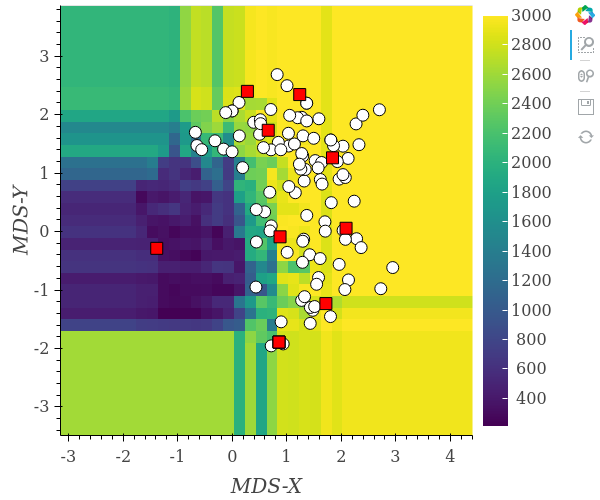
\includegraphics[width=0.5\textwidth]{configurator_footprint0}

\begin{itemize}
  \item Question: Can we visualize how a configurator samples?
  \pause
  \item Idea: Project configurations into 2d
  \pause
  \item Challenge: Projection should preserve distance\\ between configurations
\end{itemize}

\end{frame}
%----------------------------------------------------------------------
%----------------------------------------------------------------------
\begin{frame}[c]{Configurator Behavior: Configurator Footprints}

\begin{block}{Basic Algorithm}
\LinesNotNumbered
\begin{algorithm}[H]
\BlankLine
For each pair $\langle\conf_i,\conf_j\rangle$ in runhistory, compute similarity $s(\conf_i,\conf_j)$;\\
Fit $2$d $MDS$ based on similarities $s(\conf_i,\conf_j)$;\\
Replace each $\conf$ in $\hist$ by 2d projection $MDS(\conf)$;\\
Plot each $\conf$ in 2d space;\\
\caption{Configurator Footprint (Visualization of a runhistory)}
\label{algo:confvis}
\end{algorithm}
\end{block}

\pause

\begin{block}{Distance in Configuration Space $\pcs$ \litw{Xu et al.'16}}
\begin{description}
  \item[Continuous] $|\conf_i - \conf'_i| / (\conf_{i, \text{max}} - \conf_{i, \text{min}})$ 
  \item[Categorical] $0 \text{ if } \conf_i == \conf'_i \text{ else } 1$
  \item[Inactive vs Active] $1$
\end{description}

\end{block}

\end{frame}
%----------------------------------------------------------------------
%----------------------------------------------------------------------
\begin{frame}[c]{Configurator Behavior: Extended Configurator Footprints}

\begin{block}{Some Improvements}
\begin{itemize}
  \item Visualize on how many instances a configurations was evaluated
  \begin{itemize}
	\item[$\leadsto$] adapt size of dots accordingly     
  \end{itemize}
  \pause
  \medskip
  \item Highlight incumbent configurations 
  \begin{description}
	\item[upward triangle] default configuration
	\item[downward triangle] final incumbent
	\item[red squares] intermediate incumbents 
  \end{description}
  \pause
  \medskip
  \item Distinguish between random configs and EI-optimized configs
  \pause
  \medskip
  \item Highlight marginalized cost in background
  \begin{enumerate}
    \item fit EPM $\surro: \perf^2 \times \insts \to \perf$ based on runhistory
    \item Plot heatmap in background based on $\frac{1}{|\insts|}\sum_{\inst \in \insts}\surro(MDS(\conf),\inst)$
  \end{enumerate}
\end{itemize}
\end{block}

\end{frame}
%----------------------------------------------------------------------
%----------------------------------------------------------------------
\begin{frame}[c]{Configurator Behavior: Configurator Footprints}

\centering
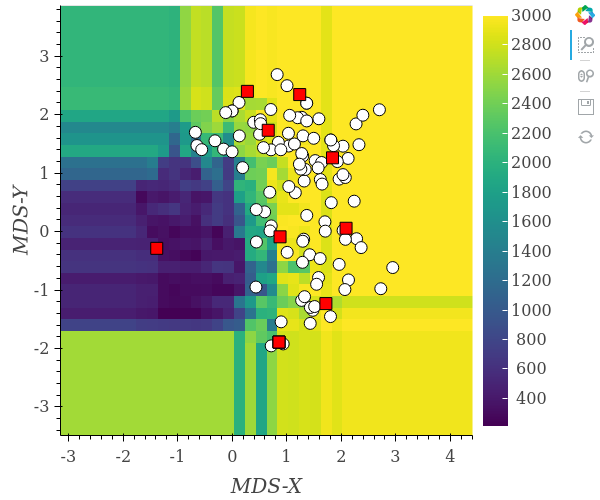
\includegraphics[width=0.7\textwidth]{configurator_footprint0}

\end{frame}
%----------------------------------------------------------------------
%----------------------------------------------------------------------
\begin{frame}[c]{Configurator Behavior: Configurator Footprints}

\centering
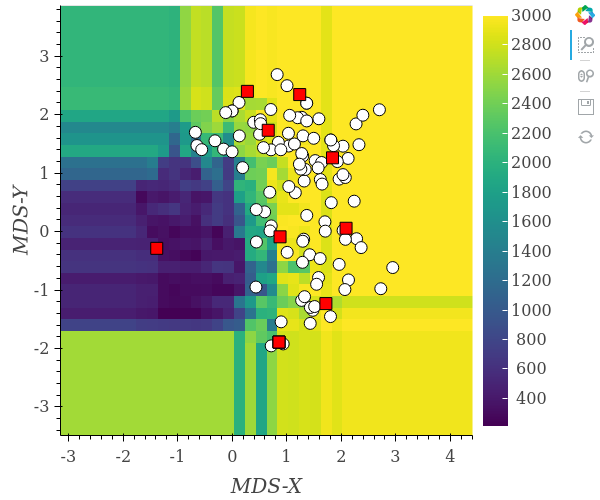
\includegraphics[width=0.31\textwidth]{configurator_footprint0}\quad
\includegraphics[width=0.31\textwidth]{configurator_footprint5}\quad
\includegraphics[width=0.31\textwidth]{configurator_footprint9}

$10\%$ of $\conf$ \hspace{2.1cm} $50\%$ of $\conf$ \hspace{2.1cm} $100\%$ of $\conf$

\bigskip
\pause

\begin{itemize}
  \item \alert{Insight I}: SMAC focuses on high-performance area
  \item \alert{Insight II}: high-performance region is quite large ($\leadsto$ easy to optimize)
\end{itemize}

\end{frame}
%----------------------------------------------------------------------
%----------------------------------------------------------------------
\begin{frame}[c]{Learning Goals}

Now, you should be able to \ldots

\begin{itemize}
  \item use data gathered for algorithm configuration to gain more insights about the algorithm and instances
  \item distinguish between global and local parameter importance
  \item explain parameter importance for the following approaches:
  \begin{itemize}
    \item fANOVA
    \item Ablation studies
    \item Forward selection
    \item Local parameter importance (LPI)
  \end{itemize}
  \item understand and use performance analysis approaches\\ (incl. algorithm footprints)
  \item understand and use configurator analysis\\ (e.g., performance over time and algorithm configurator footprints)
\end{itemize}

\end{frame}
%----------------------------------------------------------------------
%----------------------------------------------------------------------
\begin{frame}[c]{Further Literature---These are links!}

\begin{itemize}
    \item \href{http://aad.informatik.uni-freiburg.de/papers/14-ICML-HyperparameterAssessment-longversion.pdf}{fANOVA}
    \item \href{http://aad.informatik.uni-freiburg.de/papers/13-LION-FeatureAndParameterImportance.pdf}{Forward Selection}
    \item \href{http://www.cs.ubc.ca/~hoos/Publ/FawHoo13.pdf}{Ablation}
    \item \href{https://ml.informatik.uni-freiburg.de/papers/17-AAAI-Surrogate-Ablation.pdf}{Efficient Ablation}
    \item \href{https://ml.informatik.uni-freiburg.de/papers/18-LION12-CAVE.pdf}{LPI \& algorithm configurator footprints (part of the CAVE paper)}
\end{itemize}


\end{frame}
%----------------------------------------------------------------------
